\documentclass{article}
\IfFileExists{neurips_2025.sty}{\usepackage[preprint]{neurips_2025}}{%
  \usepackage[letterpaper,textwidth=5.5in,textheight=9in,top=1in]{geometry}\usepackage{times}}
\usepackage[utf8]{inputenc}
\usepackage[T1]{fontenc}
\usepackage{float}
\usepackage{hyperref,url,booktabs,amsmath,amssymb,graphicx,microtype}

\title{Generating Paintings with a Deep Convolutional GAN}
\author{Niklas Chang \\ University of California, San Diego \\ \texttt{nhchang@ucsd.edu}}

\begin{document}
\maketitle

\begin{abstract}
We train a deep convolutional generative adversarial network (DCGAN) on 15,000 paintings
from the WikiArt dataset and use it to generate new $64\times64$ paintings. We report the training
loss curves and evaluate the generated images with the Inception Score (IS) and FID.
The model reaches an IS of 2.78 and an FID of 0.048 (real paintings: 3.68 and 0.0059). Code is available at \url{https://github.com/Niklichang/ECE285-HW2}.
\end{abstract}

\section{Method}
\paragraph{Data.} We use a subset of the full Kaggle WikiArt dataset: the first 15,000 paintings (all styles) of the same WikiArt collection, downloaded from its
Hugging Face copy (\texttt{huggan/wikiart}). Images are center-cropped, resized to $64\times64$, and scaled to $[-1,1]$. During training, images are
randomly flipped horizontally.

\paragraph{Model.} A GAN trains two networks against each other. The generator $G$ maps a random
noise vector $z\sim\mathcal N(0,I)$ to an image, and the discriminator $D$ outputs the probability that
an image is real. We follow the DCGAN architecture~\cite{radford2016dcgan}: $G$ uses transposed convolutions with batch
normalization and ReLU, ending in a $\tanh$; $D$ uses strided convolutions with batch normalization and
LeakyReLU. $D$ is trained to tell real from generated images, and $G$ is trained to fool $D$:
\begin{equation}
\mathcal L_D = -\log D(x) - \log\big(1-D(G(z))\big), \qquad \mathcal L_G = -\log D(G(z)).
\end{equation}
The two networks are updated in turn, once each per batch.

\paragraph{Hyperparameters.} Table~\ref{tab:hp} lists the settings, which follow the DCGAN paper~\cite{radford2016dcgan}.

\begin{table}[H]
\centering\small
\caption{Hyperparameter settings.}\label{tab:hp}
\begin{tabular}{@{}ll@{\hspace{2em}}ll@{}}
\toprule
Image size & 64$\times$64 & Optimizer & Adam ($\beta_1=0.5$, $\beta_2=0.999$) \\
Noise dimension & 100 & Learning rate & 0.0002 (G and D) \\
Batch size & 128 & Epochs & 100 \\
Parameters & G: 3.58\,M, D: 2.77\,M & Weight init. & $\mathcal N(0, 0.02)$ \\
\bottomrule
\end{tabular}
\end{table}

\section{Results}
\paragraph{Training.} Figure~\ref{fig:loss} shows the losses and the discriminator's outputs during training
(100 epochs, 5.3 minutes on one GPU). Unlike a normal network, a GAN's losses do not steadily go down,
because each network's loss depends on how good the other one is. After the first few epochs, the losses
fluctuate around a stable level, with $D$ giving about 0.8 to real and 0.2 to generated images, so neither
network wins. Occasional spikes, such as in the last epoch (D loss 1.56), are typical of GAN training.

\begin{figure}[H]
\centering
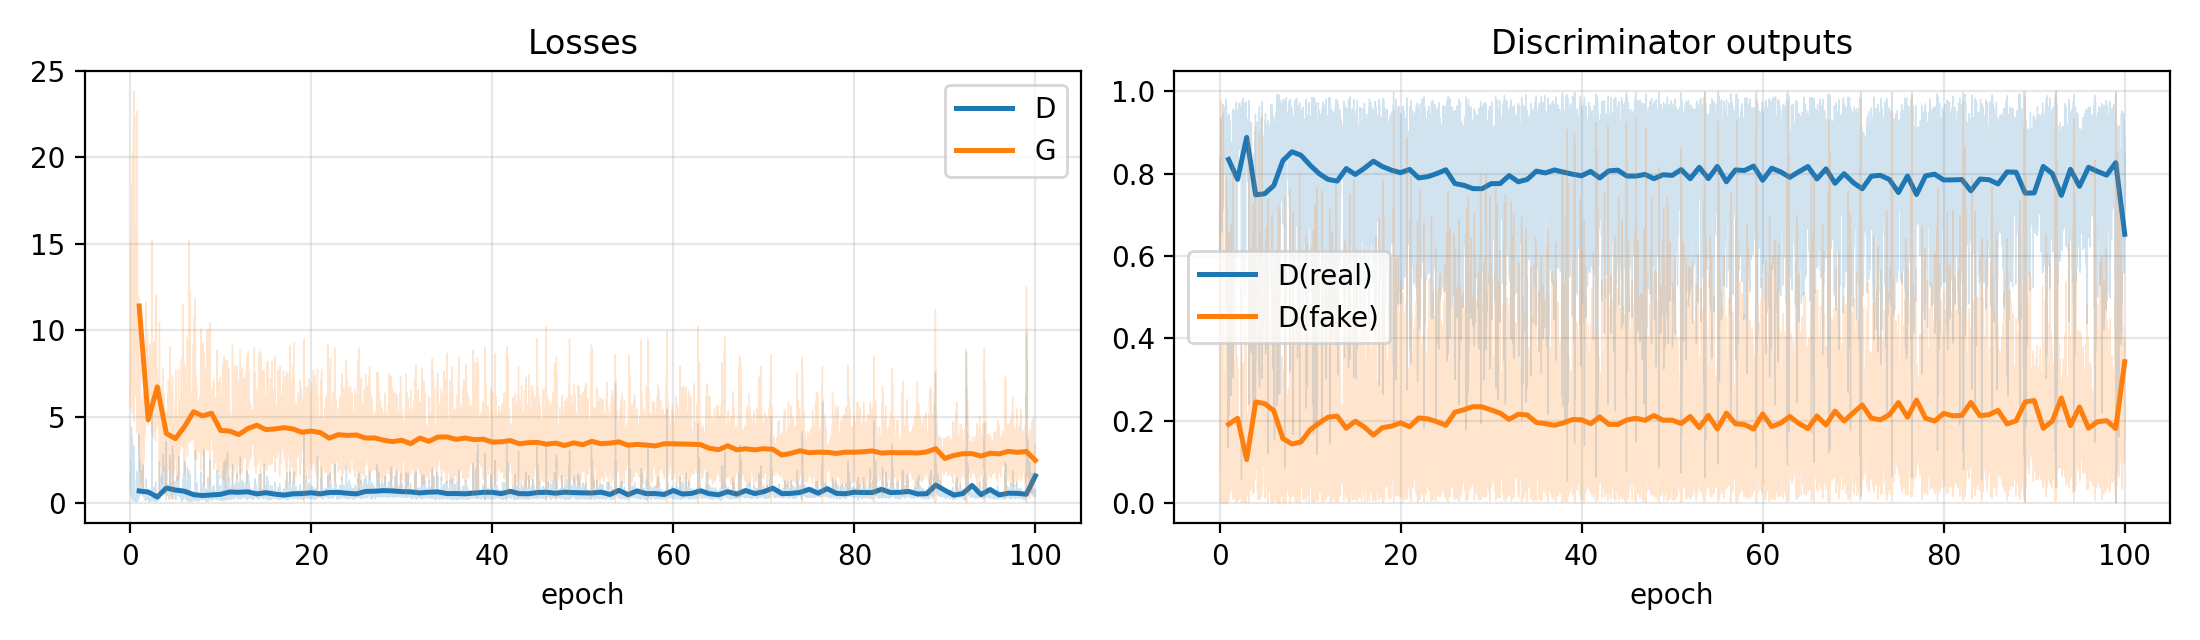
\includegraphics[width=0.95\linewidth]{loss_curves.png}
\caption{Left: discriminator and generator losses. Right: average output of $D$ on real and generated images.
Light lines are per iteration, dark lines are averages per epoch.}
\label{fig:loss}
\end{figure}

\paragraph{IS and FID.} We compute both scores with the \texttt{pytorch-ignite} code, on 7,500 generated
images compared with 7,500 real paintings. For reference, we compute the same scores for 7,500 other real
paintings (Table~\ref{tab:metrics}).

\begin{table}[H]
\centering\small
\caption{Inception Score (higher is better) and FID (lower is better).}\label{tab:metrics}
\begin{tabular}{@{}lcc@{}}
\toprule
 & IS & FID \\ \midrule
Generated paintings & 2.78 & 0.048 \\
Real paintings (reference) & 3.68 & 0.0059 \\
\bottomrule
\end{tabular}
\end{table}

\paragraph{Generated images.} Figure~\ref{fig:samples} shows generated paintings. After 1 epoch the generator only produces
blurry patterns; after training it produces images with painting-like colors, textures and compositions.

\begin{figure}[H]
\centering
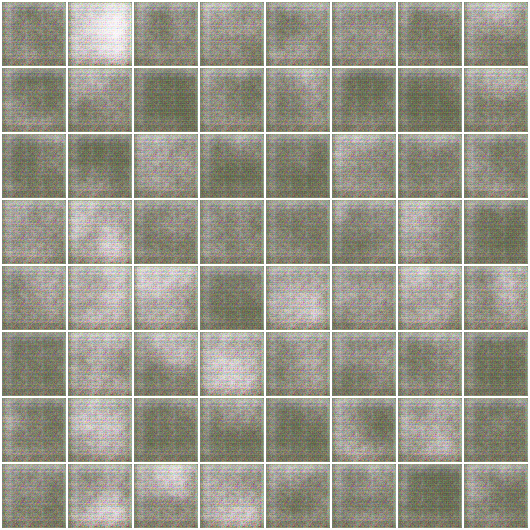
\includegraphics[width=0.45\linewidth]{samples_epoch001.png}\hfill
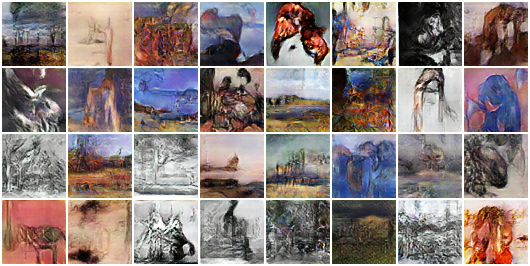
\includegraphics[width=0.45\linewidth]{samples.png}
\caption{Left: generator output after 1 epoch. Right: generated paintings after training.}
\label{fig:samples}
\end{figure}

\paragraph{Discussion.} The GAN learns the colors and textures of paintings,
but the scenes are not always coherent at $64\times64$. IS and FID use a network trained on everyday photos,
which is why we also report the scores of real paintings for comparison. Our FID values are on the scale
of the \texttt{pytorch-ignite} implementation, which is much smaller than FIDs reported in papers, so they
are only meaningful relative to the real-data reference: the generated images are clearly further from
real paintings (0.048 vs.\ 0.0059) and less diverse (IS 2.78 vs.\ 3.68).


{\small
\bibliographystyle{plain}
\bibliography{refs}}
\end{document}
